\documentclass{oci}
\usepackage[utf8]{inputenc}
\usepackage{float}

\title{El lokómon legendario}


\begin{document}
\begin{problemDescription}

Tu amigo Ashvier, un osado maestro lokómon, logró escalar hasta la cima de la montaña más alta de
la Cordillera Norte.
Tras una larga batalla, su misión ha sido todo un éxito y logró capturar al lokómon legendario Blatiaz.
% ¡Esta increíble hazaña aparecerá en los libros de historia!

Ashvier ahora debe descender y regresar al centro lokómon
% de ciudad Hiérrica
para así poder curar a sus lokómones.
Lamentablemente, su kit de alpinismo se cayó por el acantilado durante la batalla y debe buscar
una forma alternativa para descender.
Afortunadamente, su nuevo lokómon legendario Blatiaz tiene la habilidad de planear.
% Esta habilidad le permite descender desde la cima de una montaña hacia la cima
% de otra montaña de menor altura.

La Cordillera Norte está formada por $n$ montañas de diferentes alturas, distribuidas una al lado
de la otra a lo largo de una línea.
Las montañas son enumeradas de izquierda a derecha entre 0 y $n-1$.
La habilidad de Blatiaz le permite planear desde la cima de una montaña
hasta la cima de otra montaña más baja, siempre y cuando una montaña más alta no bloquee
el desplazamiento.
Dadas dos montañas en posiciones $i$ y $j$ con alturas $h_i$ y $h_j$ ($h_j < h_i$) respectivamente,
decimos que una montaña en la posición $k$ ($min(i, j) < k < max(i, j)$) \emph{bloquea} el
desplazamiento si su altura $h_k$ es mayor o igual que $h_i$.

% Es decir, si Blatiaz está en la cima de la montaña en la posición $i$, y esta tiene altura $h_i$,
% Blatiaz puede descender a la cima de la montaña en la posición $j$ con altura $h_j$, solo si
% $h_j < h_i$ y además todas las montañas en posición $k$ ($i<k <j$) cumplen
% $h_k < h_j$.

A continuación se muestra un ejemplo para $n=4$ montañas.
En la figura de la izquierda se puede apreciar que Blatiaz puede descender desde la montaña 2
hasta la montaña 0 pues esta es de menor altura.
Por el contrario, como se muestra en la figura de la derecha, no es posible descender de la
montaña 0 hacia la montaña 3 pues, a pesar de que la montaña 3 es más baja, la montaña 2 bloquea el
desplazamiento.

\begin{center}
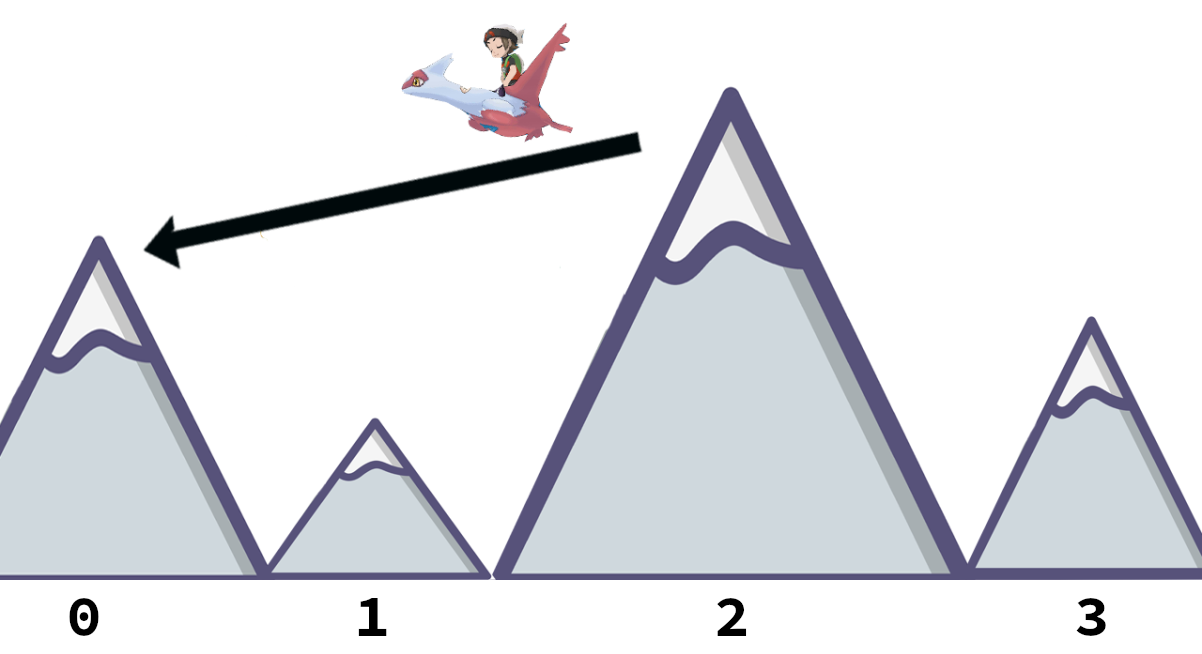
\includegraphics[width=0.48\textwidth]{allowed.png}
~
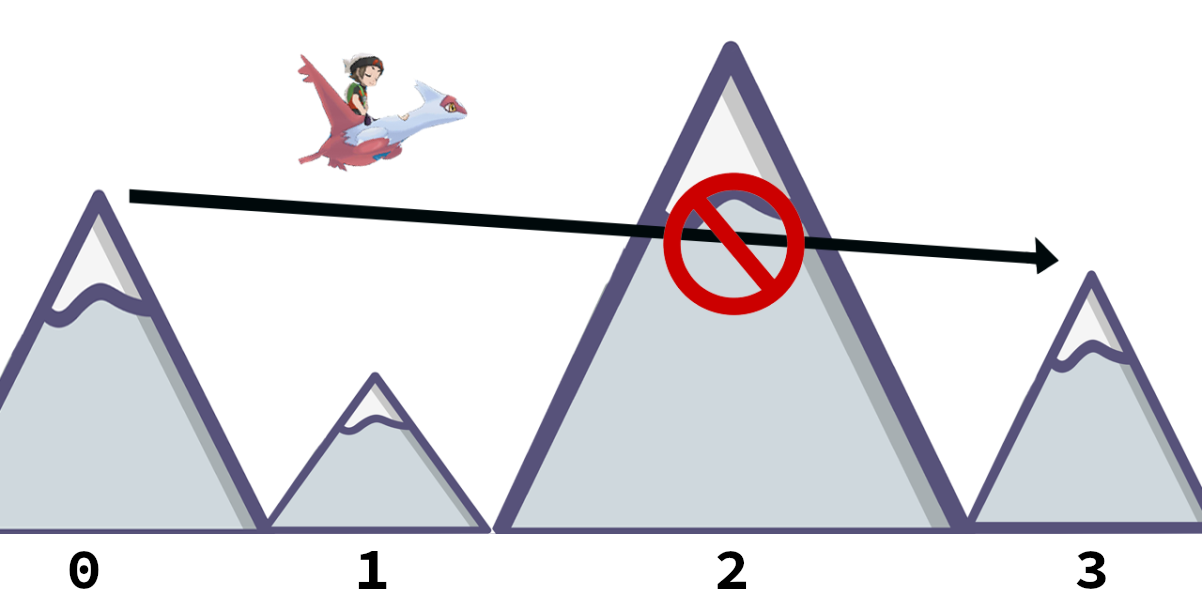
\includegraphics[width=0.48\textwidth]{disallowed.png}
\end{center}

Desde la montaña 2, Blatiaz también podría descender a las montañas 1 y 3 pero
como es su primera vez planeado sobre Blastiaz, Ashvier tomará algunas precauciones.
Partiendo de la cima de la montaña más alta, Ashvier siempre descenderá a la cima de
{\bf la montaña más alta que no esté bloqueada}.
Siguiendo este proceso, llegará a una montaña desde la cual no es posible seguir descendiendo.
Llamaremos a esta montaña la \emph{montaña final}.

Dada la descripción de las montañas, a Ashvier le gustaría saber cuál será la
montaña final.
De esta forma puede avisarle de antemano a su amigo el profesor Perezoak, quién lo estará
esperando para llevarlos al centro lokómon.
?`Podrías ayudarlos?

% Blatiaz prefiere las alturas, por lo tanto, el descenso de Ashvier está sujeto al
% siguiente procedimiento.
% Se visita la montaña más alta posible mediante la habilidad de planeo, recordando las
% condiciones establecidas.
% Se repite el paso anterior para cada nuevo trayecto.
% Si ninguna otra montaña puede ser visitada, entonces han llegado a su destino,
% en donde estará el profesor Perezoak esperándolos para llevarlos a la ciudad.

% Ashvier debe informarle de antemano al profesor Perezoak el lugar de encuentro, y,
% como buen amigo, conoce tu ingenio y destreza para resolver problemas programando,
% por lo tanto,
% te pide ayuda para crear un programa que le permita saber en qué montaña terminará su trayecto.
% Tienes a tu disposición un mapa de la Cordillera Norte, que indica la distribución espacial
% de las montañas según la altura de sus cimas.


\end{problemDescription}

\begin{inputDescription}

La entrada consiste de dos líneas.
La primera contiene un solo entero $n$ ($2 \leq n \leq 1\,000\,000$)
correspondiente al número de montañas que conforman la Cordillera Norte.
La segunda línea contiene $n$ enteros describiendo las montañas.
El primer entero corresponde a la posición de la montaña más alta, el segundo a la posición
de la segunda montaña más alta y así hasta el último entero que corresponde a la posición
de la montaña más baja.

\end{inputDescription}

\begin{outputDescription}
La salida de contener un único entero, correspondiente a la posición de la \emph{montaña final}.
\end{outputDescription}

\begin{scoreDescription}
  \subtask{30}
  Se probarán varios casos en los que $n<1000$.
  \subtask{70}
  Se probarán varios casos sin restricciones adicionales.
\end{scoreDescription}

\begin{sampleDescription}
\sampleIO{sample-1}
\sampleIO{sample-2}
\sampleIO{sample-3}
\end{sampleDescription}

\end{document}
